\chapter{中微子振荡分析方法（Oscillation Analysis Methods）}
%=====================================================================
反应堆中微子实验的核心目标是通过精确测量反中微子能谱的精细结构来提取振荡参数，并进一步判定中微子质量顺序。对于如 JUNO 这类中基线实验而言，振荡信号体现在重建能谱中的振荡起伏结构上。要可靠解析这些微小结构，必须对“从反应堆到重建谱”的完整物理与统计链条进行统一、精确且可计算的建模。任何一个环节的近似处理或数值误差，都可能在参数提取中放大为系统偏差。因此，建立一个物理自洽、并适用于大规模统计检验的分析框架，是开展后续灵敏度与覆盖率研究的基础。

本章实现了从反应堆出射谱到探测器重建能量谱的张量化谱生成链，将其分解为四个明确的矩阵/张量层次：反应堆中微子能谱（source spectrum），IBD 微分散射截面矩阵（cross-section tensor），沉积能量能谱（deposited-energy spectrum），探测器响应矩阵到重建能谱（detector response tensor）。
该张量化表达在数值上将多次卷积叠加统一为高维张量运算，大幅提升了批量计算与并行化的可行性。

本章的组织如下：第~\ref{sec:theory} 节介绍中微子产生与 IBD 及其探测；第~\ref{sec:Arrived neutrino spectrum} 节给出反应堆反中微子通量的预测方法；第~\ref{sec:Deposited energy spectrum} 节推导微分截面与沉积谱的张量化实现；第~\ref{sec:Reconstructed energy spectrum} 节详细讨论探测器响应矩阵与能量重建；第~\ref{sec:statistical method} 节描述统计拟合方法、Wilks 的适用性检验与 Feldman–Cousins 的实现要点，并总结本章为后续的灵敏度与覆盖率研究作技术铺垫。
\section{反应堆中微子的探测}
\label{sec:theory}
在商用轻水反应堆中释放的电子反中微子 $\bar{\nu}_e$ 主要来自轻水反应堆中四种主要裂变产物：$^{235}$U、$^{238}$U、$^{239}$Pu 和 $^{241}$Pu。以 JUNO 实验为例，其周围核电站提供超过 99.7\% 的中微子通量来源于上述四种核素。反应堆中微子被认为是能量在数 MeV 量级的低能中微子，其出射谱由上述各同位素的裂变率与每次裂变产生的谱形共同决定。

\begin{figure}[htbp]
\centering
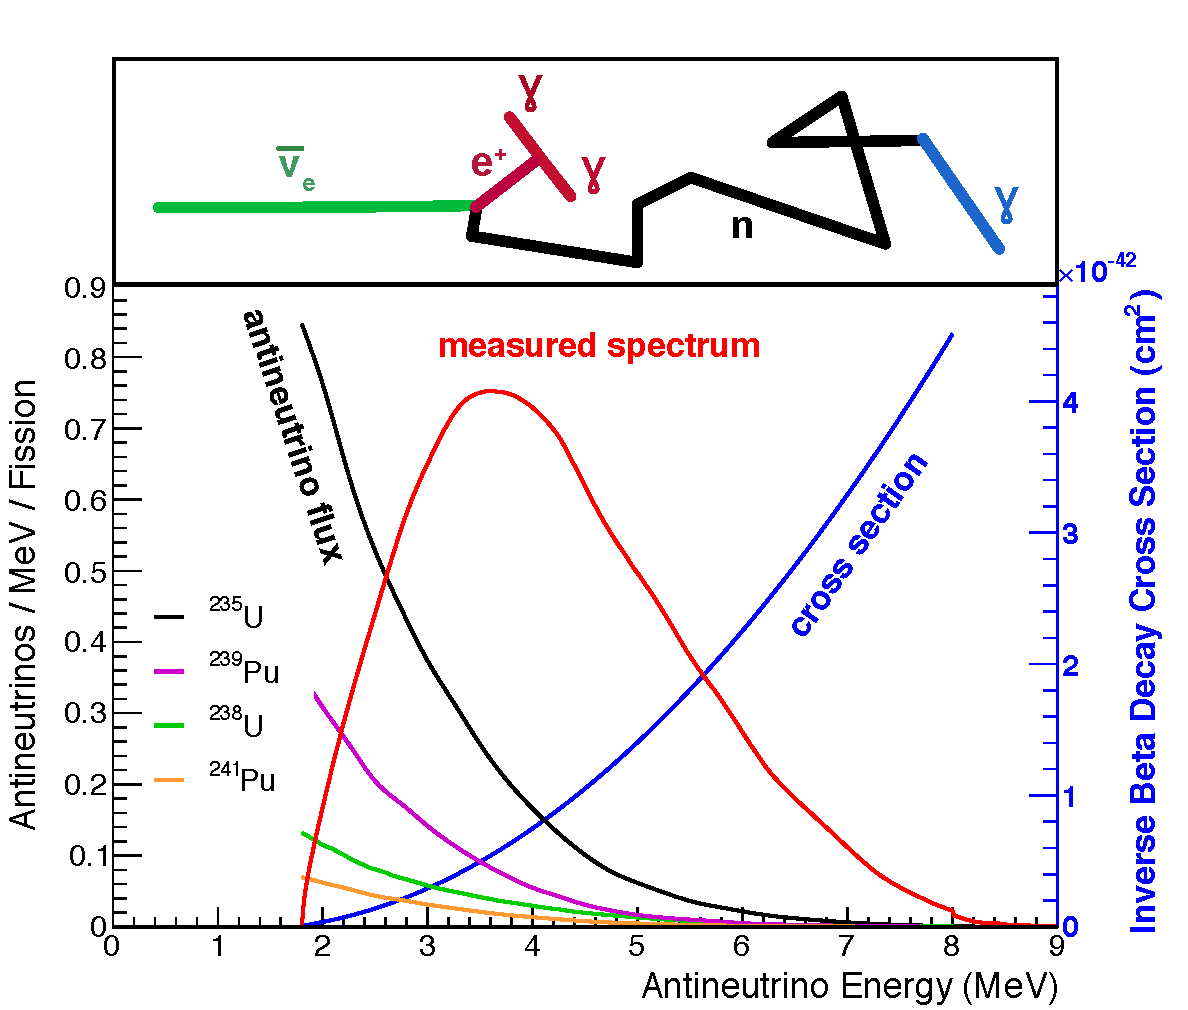
\includegraphics[width=0.9\linewidth]{Img/Figure-2.pdf}
\bicaption[通过 IBD 测得的反应堆中微子能谱与四种核素产生的中微子流强构成]{图中红线为通过逆贝塔衰变（IBD）测量得到的预期反应堆中微子预期总能谱，蓝线为 IBD 反应截面随中微子能量的变化，彩色实线分别表示四种主要裂变核素（$^{235}\mathrm{U}$、$^{239}\mathrm{Pu}$、$^{238}\mathrm{U}$、$^{241}\mathrm{Pu}$）产生的中微子谱流强。顶部示意图给出 IBD 事件的关联事例（正电子与湮灭 $\gamma$）与延迟（中子俘获 $\gamma$）的偶然符合。图来自文献\citep{Vogel2015NeutrinoOscillation}}{Expected reactor antineutrino energy spectrum measured by the IBD reaction and component contributions. The red curve shows the expected total reactor antineutrino spectrum as measured via the inverse beta decay (IBD) channel (antineutrino energy per MeV per fission). The blue curve (right axis) gives the energy-dependent IBD cross section (cm$^2$). Colored solid lines denote the antineutrino fluxes produced by the four main fissile isotopes ($^{235}\mathrm{U}$, $^{239}\mathrm{Pu}$, $^{238}\mathrm{U}$, $^{241}\mathrm{Pu}$). The schematic above illustrates the typical prompt (positron and annihilation $\gamma$) and delayed (neutron capture $\gamma$) signals of an IBD event. The figure emphasizes the IBD sensitivity in the few-MeV region and the isotope-dependent spectral features relevant for reactor neutrino spectroscopy and oscillation analyses (figure from Ref\citep{Vogel2015NeutrinoOscillation}).}
\label{fig:reactor_ibd_spectrum}
\end{figure}

图~\ref{fig:reactor_ibd_spectrum} 展示了通过 IBD 反应测得的反应堆中微子能谱（红线）、IBD 截面（蓝线）与四种主要裂变核素的通量贡献（彩色曲线）；该图说明了不同核素对谱形的差异性以及IBD反应示意，因而精确的能量重建与谱学系统误差控制对振荡参数与质量顺序的测定至关重要。JUNO 探测器正是通过探测这些反应堆中微子与 LS 中自由质子的 IBD 相互作用，从而获取反应堆中微子通量和能谱信息，为中微子振荡参数的精确测定提供重要数据支撑。

在基于反应堆的中微子实验中，能量在数兆电子伏特（MeV）范围内的电子反中微子（$\bar{\nu}_e$）主要通过反贝塔衰变（Inverse Beta Decay，IBD）过程进行探测，即：

\begin{equation}
\bar{\nu}_e + p \rightarrow e^+ + n 
\end{equation}

该过程通常在液体闪烁体（Liquid Scintillator, LS）探测器中发生，得益于 IBD 相对较大的反应截面，这种探测方式具有优异的灵敏度和背景抑制能力。在这一反应中，反中微子与探测介质中的自由质子相互作用，产生一个正电子和一个中子。正电子在极短时间内将其动能通过电离损失沉积于探测器中，并与电子发生湮灭反应，释放出两个 511 keV 的伽马光子，形成“快信号”（prompt signal）；而中子经过热化过程后被周围的原子核俘获，随后释放出特征性的伽马光子，形成数百微秒尺度的“慢信号”（delayed signal）。快慢信号在时间和空间上的关联性可有效抑制自然放射本底和宇生粒子等非关联事例，因而 IBD 通道在实际实验中被广泛采用，尤其适用于反应堆中微子的精准测量与振荡研究。

在 IBD 相互作用中，正电子携带了绝大部分反中微子的能量。其动能通过在闪烁体中的沉积和湮灭产生闪烁光，进而被光电倍增管（PMTs）收集转换为光电子（photoelectrons, PE），再由电子学系统记录。由于正电子能量和入射中微子能量之间存在线性关系，且快信号具有良好的时间分辨，正电子能谱可作为反中微子能谱的有效代理量。然而，探测系统的非线性响应效应（nonlinearity, NL），包括闪烁体的非线性发光、切伦科夫光的贡献，光子传播过程的损耗以及电子学系统的增益不均等，会引起实际可见能量 $E^{\text{vis}}$ 与真实能量 $E_{\bar{\nu}_e}$ 之间的偏离。因此，实验中通常采用标定源（如 $\gamma$、$e^-$ 或 $\alpha$）进行能量响应刻度，并建立非线性修正模型。

以 JUNO 为例，其液体闪烁体的组分与大亚湾实验极为相似，实验利用精细的刻度系统和基于大亚湾经验的非线性模型，对能量响应进行了全面刻画。此外，JUNO 采用优化的能量重建算法和统计方法，实现了优异的能量分辨能力。这使得其能够高精度测量正电子的沉积能量谱，进而反推出反应堆中微子能谱，在中微子质量有序、混合角精确测量等物理目标上具有显著优势。

在此介绍本分析中在能量转换中使用的各个物理量以避免模糊。当中微子进入到液体闪烁体中，会产生正电子。中微子能量$E_{\bar{\nu}_e}$会转换为正电子能量$E_e$，这一过程与粒子散射的运动学相联系。正电子能量$E_e$是中微子与正电子散射角$cos\theta$与中微子能量$E_{\bar{\nu}_e}$的函数。当正电子发生堙灭时，其总能量换转换为沉积能量$E_{dep}$。考虑液闪非线性以及淬灭效应的影响，沉积能量$E_{dep}$转换为了可见能量$E_{vis}$。随后考虑探测器响应，可见能量$E_{vis}$转换为了重建能量$E_{dep}$。

\begin{equation}
\begin{aligned}
E_{\bar\nu_e}
&\xrightarrow{\text{kinematics}}
E_e(E_{\bar\nu_e},\cos\theta)
\xrightarrow{\text{annihilation}}
E_{\rm dep}(E_e)
\\
&\xrightarrow{\text{LS nonlinearity}}
E_{\rm vis}(E_{\rm dep})
\xrightarrow{\text{resolution}}
E_{\rm rec}(E_{\rm vis}) \, .
\end{aligned}
\end{equation}


重建能量能谱的计算见下式：

\begin{multline}
\phi(E_{\text{rec}}) = \int_{T_{\text{DAQ}}} \! \mathrm{d}t \int_{1.8\,\text{MeV}}^{15\,\text{MeV}} \! \mathrm{d}E_{\bar{\nu}_e} \, \phi(E_{\bar{\nu}_e}, t) \int_{-1}^{1} \! \mathrm{d}\cos\theta \, \frac{\mathrm{d}\sigma}{\mathrm{d}\cos\theta}(E_{\bar{\nu}_e}, \cos\theta) \cdot N_p \cdot \epsilon(E_{\text{dep}}) \cdot {} \\
\frac{1}{\sqrt{2\pi} \sigma_{E_{\text{vis}}}} \exp\left[-\frac{1}{2} \left(\frac{E_{\text{vis}} - E_{\text{dep}}}{\sigma_{E_{\text{vis}}}} \right)^2 \right]
\label{eq:phi-Erec-integral}
\end{multline}

其中：
$\phi(E_{\bar{\nu}_e}, t)$是时间间隔$t$时在探测器处的经振荡后的反应堆反中微子通量。$E_{\text{dep}} = E_{\text{dep}}(E_{\bar{\nu}_e}, \cos\theta)$ 表示由中微子能量和角度确定的沉积能量；$N_p$ 是靶质子数；$\epsilon(E_{\text{dep}})$ 是探测器对沉积能量的效率；$\sigma_{E_{\text{vis}}}$ 是探测器能量分辨。

为了将反应堆产生的反中微子能谱转化为实验中观测到的重建能谱，需要经过两个主要过程的卷积。首先，反中微子在探测器中与靶质子发生反应，按照微分散射截面 $\frac{d\sigma}{d\cos\theta}$ 分布产生一系列沉积能量事件，从而得到沉积能谱。该过程还包含了靶粒子数 $N_p$ 以及探测器效率 $\epsilon(E_{\text{dep}})$ 的影响。随后，沉积能谱再通过与探测器的能量响应函数（通常近似为高斯分布）进行卷积，最终得到重建能量谱 $S(E_{\text{vis}})$。这一过程在数学上体现为三重积分，分别对应中微子能量、角度散射以及探测器响应的卷积关系。
\subsection{JUNO的核反应堆}

JUNO 实验所探测的反应堆反中微子主要来自华南地区多个商用核电站。目前，对 JUNO 贡献最显著的是台山核电站和阳江核电站，如图\ref{fig:JUNO_location}所示，共包含八个反应堆堆芯。这些堆芯到探测器的基线长度集中在约 50 km 附近，其平均距离约为 52.5 km，使其成为 JUNO 进行中微子振荡精密测量的主要信号来源。
除上述主反应堆群之外，距离JUNO稍远的大亚湾核电站以及防城港核电站作为次要反应堆源也被纳入反应堆反中微子通量的计算。其反中微子通量不可忽略，因此在本分析中予以考虑。
台山、阳江以及大亚湾各反应堆堆芯的热功率、到探测器的距离以及对应的反 IBD 事例率，已在表 2-2 中进行了系统汇总。对于距离约 265 km 的惠州核电站，由于其仍处于建设阶段，预计将在 JUNO 开始运行后的数年内才具备发电条件，且具体时间表尚存在不确定性，因此未将其纳入本工作的主要物理结果分析中。
其余距离超过 500 km 的核电站对 JUNO 的反应堆反中微子事例率贡献较小，合计约为每天一个 IBD 事例量级。在本分析框架下，这部分超过 500 km 的远距离反应堆产生的反中微子被视为一种本底分处理。关于反应堆反中微子通量的计算方法及其相关系统不确定性，将在第 2.3 节中作进一步讨论。
\begin{figure}[htbp]
  \centering
  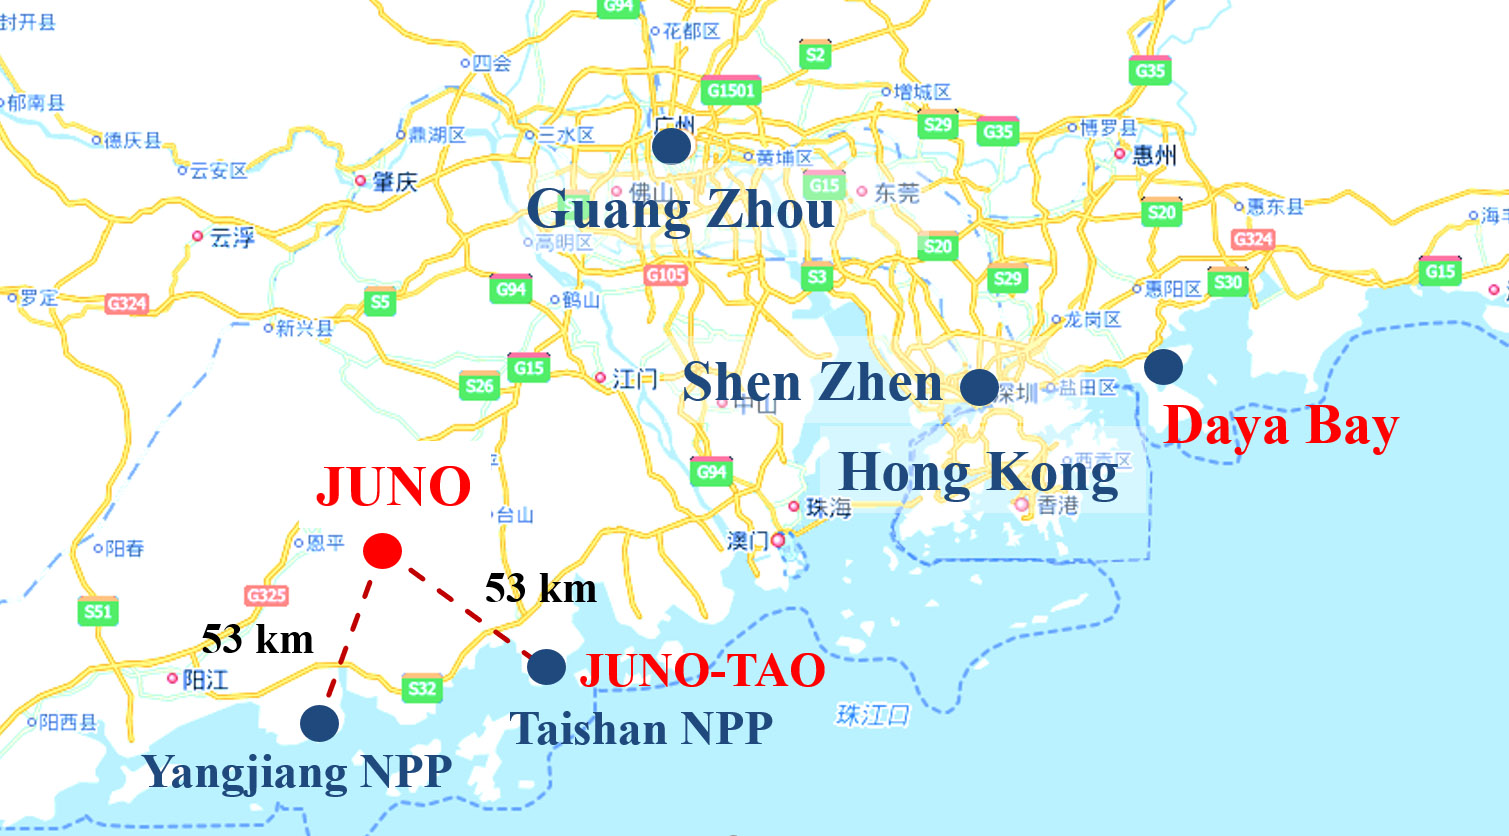
\includegraphics[width=0.9\linewidth]{Img/JUNO_location.jpg}
  \bicaption[JUNO探测器的位置]{JUNO探测器的位置}{JUNO detector location}
  \label{fig:JUNO_location}
\end{figure}

\subsection{反应堆反中微子通量的预测}
\label{sec:Arrived neutrino spectrum}

\subsubsection{反应堆反中微子能谱模型}
在商用轻水反应堆中，释出的电子反中微子主要来自若干主要裂变同位素的 β 衰变。为了构造到达探测器的中微子通量谱，常用两类方法：一种是基于转换法（conversion）得到的经验谱模型（代表性工作为 Huber–Müller 的基准谱）；另一种是基于裂变产物$\beta$支级信息的求和法（summation method），后者能够在理论上产生更丰富的谱形细节。本文以 Huber–Müller 模型作为基准反应堆谱用于生成参考到达谱，并以求和法产生的谱用于不确定度估计与谱形敏感性研究。本章分析中以 Huber–Müller 模型作为基准反应堆反中微子能谱模型，用以生成基准到达谱并作为后续不确定度评估和比较的参照。在后续不确定度量化与分 bin 策略研究中，将介绍 summation 法产生的带有精细结构的反应堆反中微子能谱模型。

对第 $r$ 个反应堆堆芯在时刻 $t$ 的中微子产额谱，可表示为
\begin{equation}
\phi_r(E_{\bar\nu},t)
= \frac{W_r(t)}{\sum_i f_{ir}(t)\,e_i}\sum_i f_{ir}(t)\,s_i(E_{\bar\nu}),
\label{eq:phi-r-reactor-spectrum}
\end{equation}
其中 $W_r(t)$ 为第 $r$ 个堆芯在时刻 $t$ 的热功率，$f_{ir}(t)$ 表示在时刻 $t$ 第 $r$ 个堆芯中第 $i$ 种裂变同位素的裂变份额（例如 $^{235}\mathrm{U}$、$^{238}\mathrm{U}$、$^{239}\mathrm{Pu}$、$^{241}\mathrm{Pu}$），$e_i$ 为第 $i$ 种裂变同位素每次裂变释放的平均能量，$s_i(E_{\bar\nu})$ 为第 $i$ 种裂变同位素每次裂变产生的反中微子能谱（基准由 Huber--Müller 给出或由求和法计算）。将各堆芯的到达谱按距离衰减与振荡概率叠加，可得探测器处的总到达通量：
\begin{equation}
\Phi(E_{\bar\nu},t)=\sum_r \frac{\phi_r(E_{\bar\nu},t)}{4\pi L_r^2}\,P_{\bar\nu_e\to\bar\nu_e}(E_{\bar\nu},L_r),
\label{eq:Phi-total-reactor-flux}
\end{equation}
其中 $L_r$ 为第 $r$ 个堆芯到探测器的基线距离， $P_{\bar\nu_e\to\bar\nu_e}$ 为电子反中微子的生存概率。

需要强调的两个额外修正项是：非平衡态（Non-Equilibrium, Non-Eq）与已乏燃料（Spent Nuclear Fuel, SNF）的贡献。一般地，堆芯中的短寿命裂变产物在开机初期或换料后并不处于完全稳态，这些非平衡贡献会在谱的若干能段产生小的附加分量；而乏燃料储存池中残余放射性也会向背景能谱提供长期、能谱上可辨的微小贡献。两者通常作为谱形的微小校正并入 $\phi_r$ 或作为独立项加入系统误差评估中（在高精度谱拟合和不确定度量化中不可忽略）。

\paragraph*{非平衡态（Non-Eq）}：部分裂变产物具有较长的半衰期（从数天到数年不等），因此在堆芯运行、功率变动或换料周期内，这些长寿命核素在瞬时并不处于生产与衰变的平衡态。它们的累积与衰变会在某些能段上产生额外的 $\beta$ 衰变贡献，从而在瞬时反中微子谱上引入能量依赖的微小修正。经验与文献研究表明，非平衡态对瞬时总通量的一般相对影响为亚百分比量级（常取约 $\sim 0.5$--$0.8\%$ 作为参考值）\citep{Huber2011_nonEq,PhysRevLett.134.201802}，但其谱形并非平坦，而是随能量呈小幅结构变化，因此在高精度谱拟合中不能完全忽略。

\paragraph*{乏核燃料（SNF）}：从堆芯卸下并置于冷却池的乏核燃料仍含大量长寿命裂变产物，若干同位素的 $\beta$ 衰变端点能量超过 IBD 反应阈值，因而在冷却过程中继续向周围环境（以及近场探测器方向）贡献微弱的反中微子通量。通过厂方的换料历史与 SNF 清单，识别出对 IBD 区间有贡献的长寿命同位素并对其剩余活度进行时间积分，是评估 SNF 贡献的标准做法。典型估计表明，SNF 对探测器的日平均通量贡献亦处于亚百分比量级（文献常给出约 $\sim 0.2$--$0.4\%$ 作为参考值）\citep{Ma2015_SNF,PhysRevLett.134.201802}，但在谱低能端或特定能段上其影响可相对放大，需在精密分析中考虑并作为系统不确定度来源之一。对于 SNF 贡献的详细计算方法及其在反应堆中微子通量中的作用，可参考 X. B. Ma 等人针对 Daya Bay 乏燃料贡献的研究\citep{Ma2015_SNF}

为将上述修正纳入基准谱，可写成
\begin{equation}
\phi_r^{\rm tot}(E_{\bar\nu},t)
= \phi_r^{\rm base}(E_{\bar\nu},t)
+ \phi_r^{\rm NonEq}(E_{\bar\nu},t)
+ \phi_r^{\rm SNF}(E_{\bar\nu},t),
\label{eq:phi-r-tot}
\end{equation}
其中 $\phi_r^{\rm base}$ 通常采用 Huber–Müller 或求和法得到的基准谱，$\phi_r^{\rm NonEq}$ 由对堆内长寿命产物的累积计算得到，$\phi_r^{\rm SNF}$ 则由冷却池中各 SNF 批次的残余放射性与几何-时间积分得到。上述两项修正既可作为谱的确定性修正项直接加入 $\phi_r^{\rm tot}$，也可在不确定度评估中作为可变项（例如通过生成一组扰动谱进行 toy-MC）来量化它们对振荡参数拟合结果的影响。

\subsubsection{反应堆相关输入不确定度处理}
在本研究中，我们对来自反应堆输入（Non-Eq、SNF、裂变能 $e_i$、裂变份额 $f_{ir}$ 等）的不确定度采取较为保守的处理方案。

1. \textbf{Non-Eq 与 SNF 的产额不确定度}

非平衡态（Non-Eq）与乏核燃料（SNF）对瞬时通量的相对影响本就处于亚百分比量级，但由于其估计具有较大模型与历史依赖性，本研究对这两类产额项采用保守置信区间：产额不确定度取 $30\%$（作为参考值并与文献/合作组当前实践一致）。在相关性处理上，Non-Eq 与 SNF 的产额不确定度在同一核电站（NPP）内部的各堆芯之间视为\textbf{完全相关}（即堆芯间该项同符号、同幅度浮动），而不同核电站之间视为\textbf{不相关}。对远场（contribution small）核电站，可将其作为平滑背景项处理，并在协方差矩阵中加入相应的方差分量。

2. \textbf{裂变能 $e_i$ 的不确定度}

裂变能 $e_i$ 定义为每次裂变最终以热功形式释放出来（已扣除中微子所带走的能量与被非裂变材料俘获的能量）。裂变能并非绝对常数，会随燃料组成、温度与中子谱出现微小变化。本文采用的近似平均值为（单位 MeV）：${}^{235}\mathrm{U}:202.36,\; {}^{238}\mathrm{U}:205.99,\; {}^{239}\mathrm{Pu}:211.12,\; {}^{241}\mathrm{Pu}:214.26$。为反映其不确定性，我们在构建总协方差矩阵时将裂变能的不确定度按“堆芯内部完全相关”的假设加入协方差（即在同一 NPP 内各堆芯归一化因子受同一裂变能波动影响）；不同 NPP 之间则视为不相关。裂变能对通量的作用主要通过归一化因子 $\sum_i f_{ir}(t)\,e_i$ 将热功 $W_r(t)$ 转换为裂变率，因此其不确定度可直接映射为谱的整体归一化不确定度。

3. \textbf{裂变份额 $f_{ir}(t)$ 的不确定度与相关性}

裂变份额随燃耗（burn-up）演化而显著变化，决定了各同位素对源谱的相对贡献。堆芯演化通常通过经过验证的燃料演化代码（如 APOLLO2/SCIENCE）结合运行与换料历史进行预测；Daya Bay 等实验证实这些预测与测量之间的偏差通常小于 $\sim 5\%$。基于此与合作组常用的经验，本文对单个同位素裂变份额取\textbf{相对不确定度 5\%}。在相关性处理上，裂变份额的不确定度在同一堆芯内部的不同同位素之间通过构造适当的相关矩阵反映（negative-correlation 等约束可强制总和守恒）；在堆芯间我们同样沿用保守策略：把裂变份额的不确定度在同一 NPP 内假定\textbf{完全相关}，不同 NPP 之间视为不相关。

除基准的 Huber–Müller 模型外，基于核数据库的求和法（summation method）能生成包含更多精细结构信息的能谱，这类谱对于评估反应堆模型依赖引入的系统误差尤为重要。因此，在后续的不确定度量化与分 bin 策略研究中，将同时使用 Huber–Müller 基准谱与由 summation 法产生的一组扰动谱作为输入，评估对振荡参数拟合的影响。


\begin{table}[!htbp]
  \bicaption[JUNO 主要反应堆堆芯信息（功率、基线与裂变份额）]{本表列出用于本文分析的主要反应堆堆芯信息，包括堆芯标识（CoreName）、所属核电站（NPP）、额定热功率（GW）、到 JUNO 的基线距离（km），以及四种主要裂变同位素 $^{235}\mathrm{U}$、$^{238}\mathrm{U}$、$^{239}\mathrm{Pu}$ 和 $^{241}\mathrm{Pu}$ 的裂变份额 $f_{235}$, $f_{238}$, $f_{239}$, $f_{241}$。裂变份额 $f_i$ 表示在给定时刻该堆芯裂变中由同位素 $i$ 贡献的相对比例，其数值随燃料燃耗演化而变化，本表给出为某一参考时刻的代表性取值。DYB（Daya Bay）与 FangChengGang（防城港）为远场反应堆群，其基线较远，对 JUNO 的贡献在本文中作为次要成分处理。}{This table lists the main reactor core information used in this analysis, including core identifier (CoreName), nuclear power plant (NPP), rated thermal power (GW), baseline distance to JUNO (km), and the fission fractions $f_{235}$, $f_{238}$, $f_{239}$, $f_{241}$ of the four main fission isotopes $^{235}\mathrm{U}$, $^{238}\mathrm{U}$, $^{239}\mathrm{Pu}$, and $^{241}\mathrm{Pu}$. The fission fraction $f_i$ denotes the relative contribution of isotope $i$ to fissions in that core at a given time; it evolves with fuel burn-up, and the values given here are representative at a reference time. DYB (Daya Bay) and FangChengGang are distant reactor groups; their baselines are large and their contributions to JUNO are treated as secondary in this analysis.}
  \label{tab:reactor_cores}
  \centering
  \footnotesize
  \setlength{\tabcolsep}{4pt}
  \renewcommand{\arraystretch}{1.2}
  \begin{tabular}{@{}l l r r r r r r@{}}
    \toprule
    CoreName & NPP & Power (GW) & Baseline (km) & $f_{235}$ & $f_{238}$ & $f_{239}$ & $f_{241}$ \\
    \midrule
    TS\_C1   & TS  & 4.09  & 52.77 & 0.67 & 0.08 & 0.22 & 0.03 \\
    TS\_C2   & TS  & 4.15  & 52.64 & 0.46 & 0.08 & 0.37 & 0.08 \\
    YJ\_C1   & YJ  & 1.91  & 52.74 & 0.55 & 0.07 & 0.30 & 0.07 \\
    YJ\_C2   & YJ  & 2.74  & 52.82 & 0.59 & 0.08 & 0.29 & 0.05 \\
    YJ\_C3   & YJ  & 2.86  & 52.41 & 0.50 & 0.08 & 0.35 & 0.07 \\
    YJ\_C4   & YJ  & 1.55  & 52.49 & 0.72 & 0.07 & 0.18 & 0.03 \\
    YJ\_C5   & YJ  & 2.47  & 52.11 & 0.58 & 0.08 & 0.30 & 0.05 \\
    YJ\_C6   & YJ  & 2.87  & 52.19 & 0.51 & 0.08 & 0.34 & 0.07 \\
    DYB\_6Cs & DYB & 15.90 & 215.00 & 0.55 & 0.08 & 0.31 & 0.06 \\
    FCG\_4Cs & FangChengGang & 9.28 & 411.00 & 0.58 & 0.07 & 0.30 & 0.05 \\
    \bottomrule
  \end{tabular}
\end{table}



为了获得到达探测器处的反中微子能谱，需将修正后的反应堆发射谱与反中微子在传播过程中发生振荡的存活概率 $P_{ee}(E_\nu, L_{dr})$ 相乘，其中 $L_{dr}$ 为反应堆 $r$ 到探测器 $d$ 的基线长度：
\begin{equation}
\phi_{r}(E_\nu, t) = \phi_r'(E_\nu,t) \cdot P_{ee}(E_\nu, L_{r})
\label{eq:phi-r-at-detector}
\end{equation}
此处中微子在物质中的传播将受到物质效应的影响，这由 Wolfenstein 最早提出~\cite{Wolfenstein1978}，并由 Mikheyev 和 Smirnov 进一步发展~\cite{Mikheyev1985}。因此$P_{ee}$ 包含了由中微子与地壳电子相互作用所引起的物质效应~\cite{Akhmedov2004}。


当反中微子在基线 $L_{dr}$ 上传播至探测器 $d$ 时，其味态成分根据上式中三种轻子味的振荡公式发生演化 带有物质效应的反中微子存活概率见图~\ref{fig:osc_prob}。

\begin{figure}[htbp]
\centering
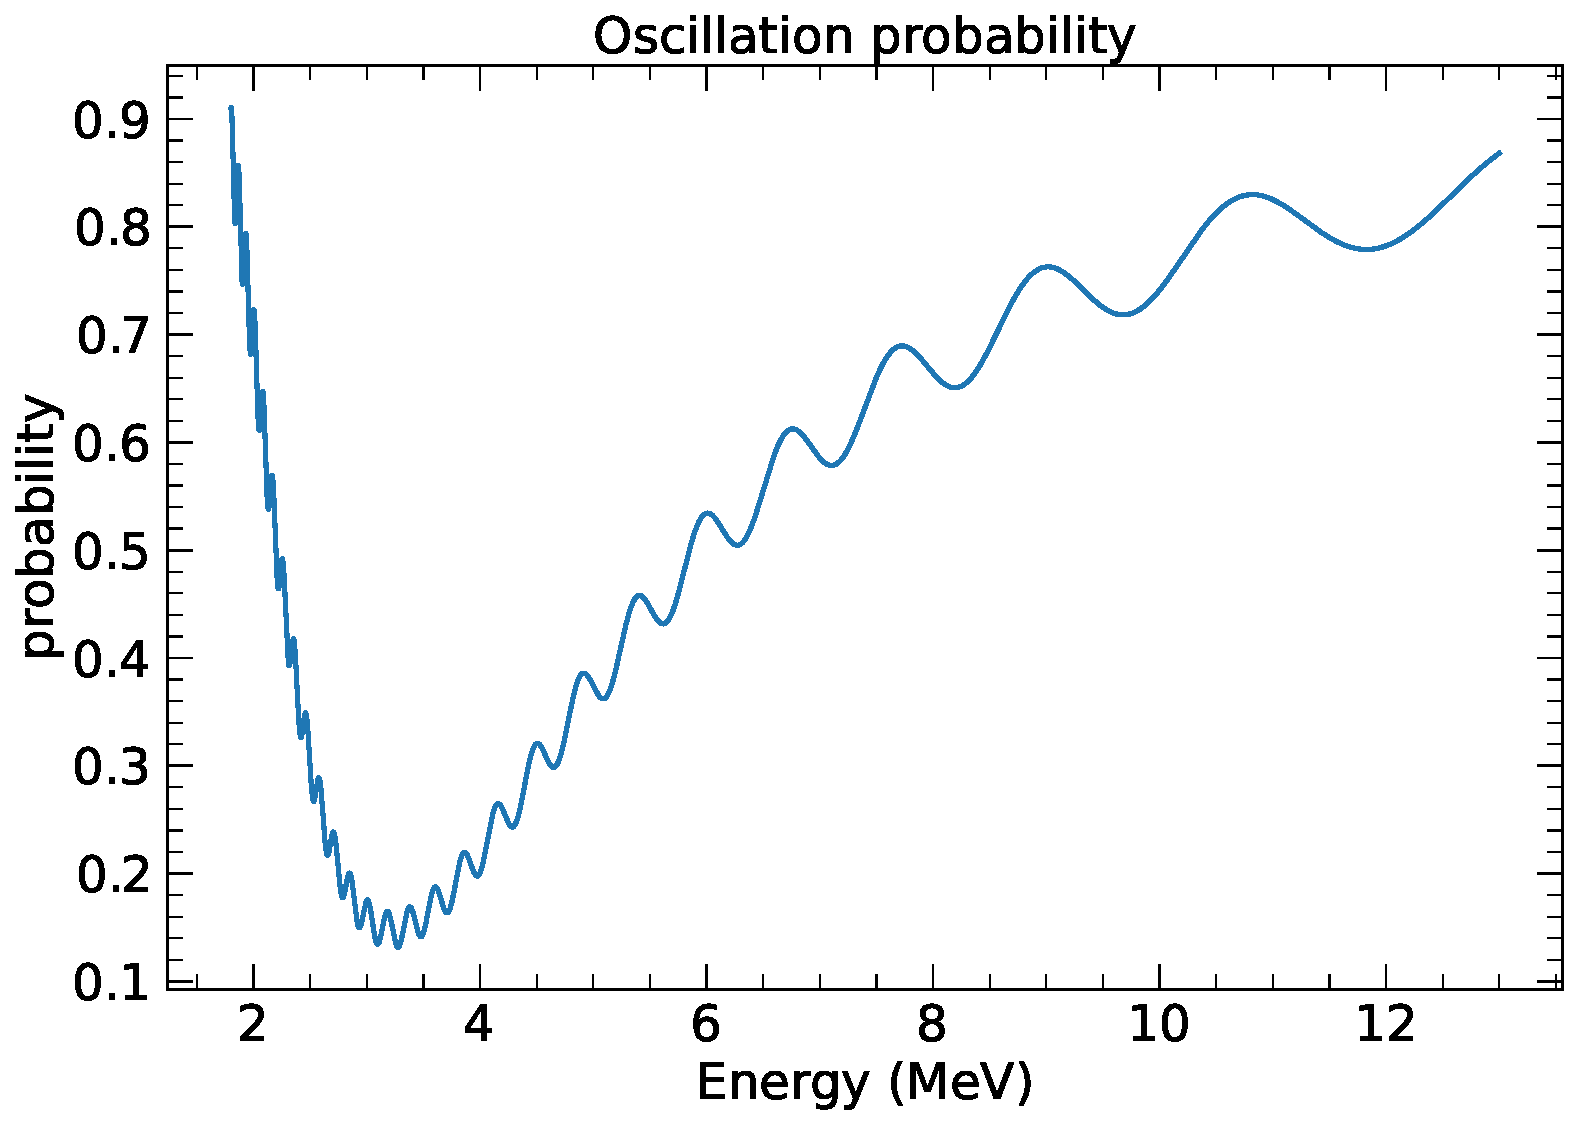
\includegraphics[width=0.6\textwidth]{Img/spectrum_cal/Oscillation_probability.pdf}
\bicaption{反中微子存活概率}{Electron antineutrino survival probability}
\label{fig:osc_prob}
\end{figure}

综上所述，通过引入乏燃料效应、非平衡修正及大亚湾经验修正因子，得到了更加精确的反应堆发射反中微子能谱 $\phi_r'(E_\nu,t)$。如图~\ref{fig:reactor_nu_arrival}，显示了核反应堆在裂变产物加权下的出射反中微子能谱（未考虑振荡），它作为后续到达谱与振荡折算的基准输入；进而结合恒定密度近似下的三味中微子振荡概率 $P_{ee}(E_\nu, L_r)$，可以计算得到到达探测器处的反中微子能谱 $\phi_{r}(E_\nu,t)$。  
如图~\ref{fig:reactor_nu_spectrum} 所示，将图~\ref{fig:reactor_nu_arrival}的出射谱与图~\ref{fig:osc_prob}中振荡概率以及几何衰减 $1/4\pi L^2$ 相乘后得到的实际到达探测器的能谱；加入振荡效应后，能谱中出现了随能量变化的振荡结构，反映了中微子质量本征态与味态之间的混合及传播演化行为。

\begin{figure}[ht]
  \centering
  \begin{subfigure}[t]{0.47\textwidth}
    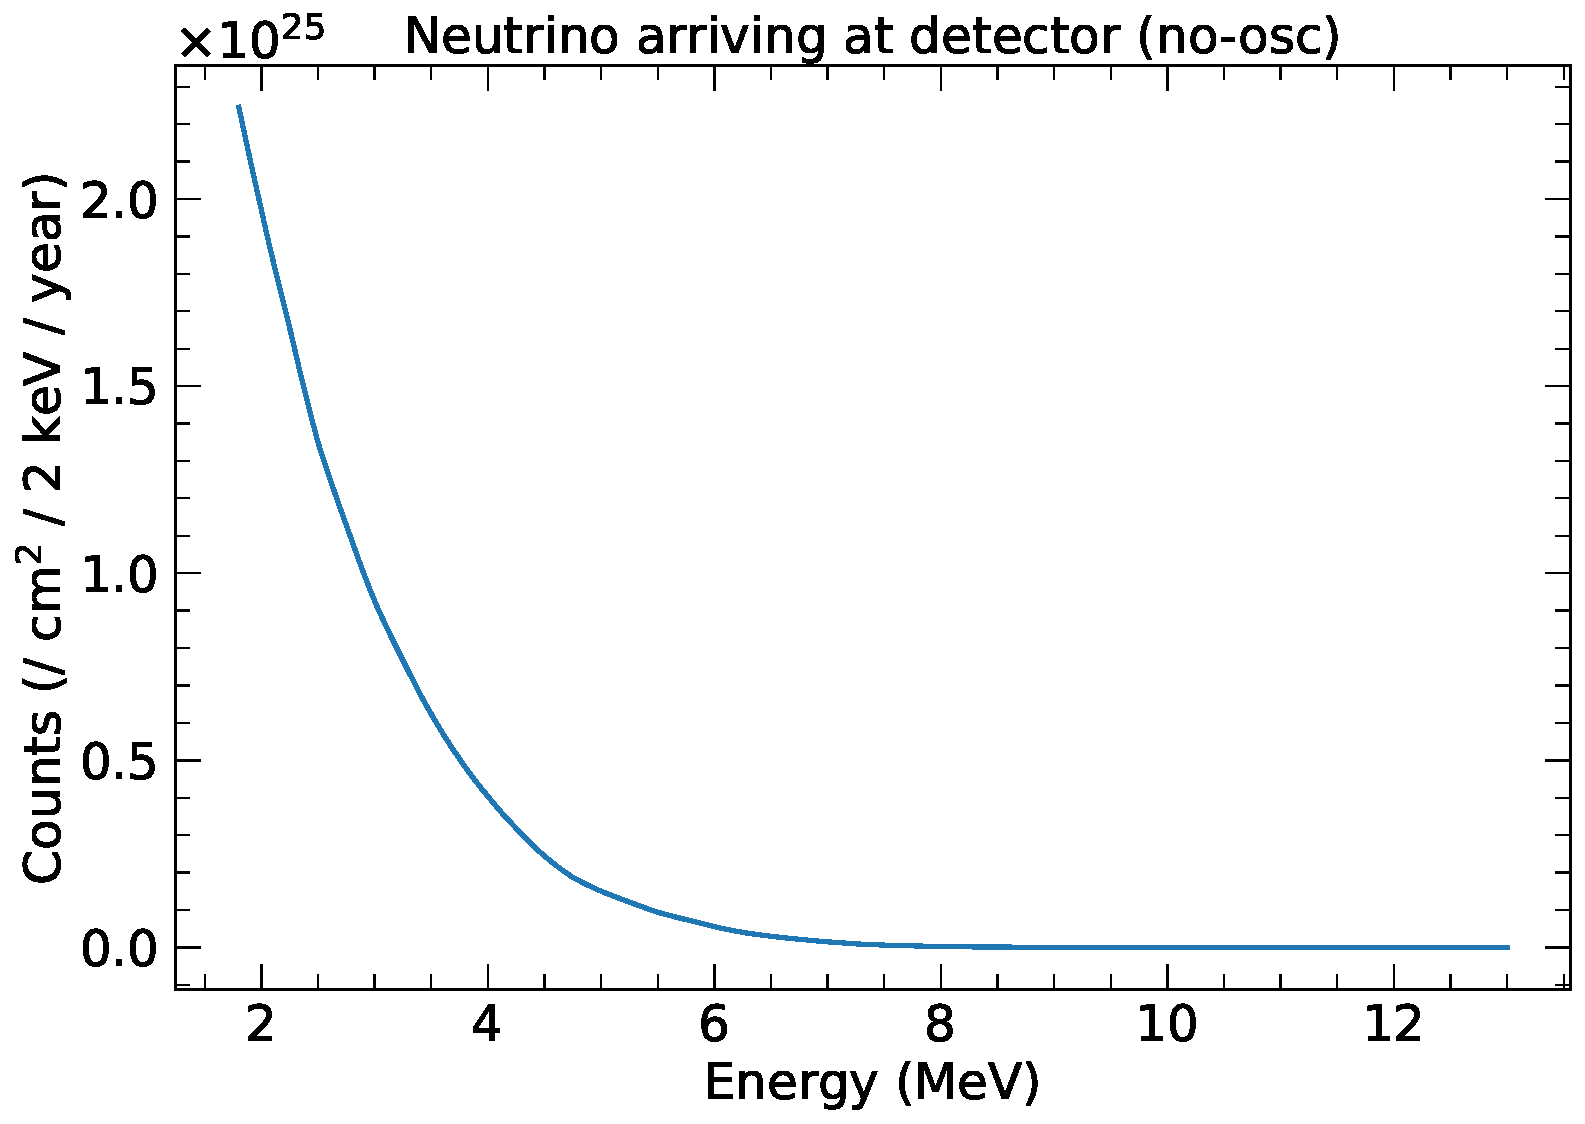
\includegraphics[width=\textwidth]{Img/spectrum_cal/Neutrino_arriving_at_detector.pdf}
    \caption{反应堆发射谱（未加振荡）}
    \label{fig:reactor_nu_arrival}
  \end{subfigure}%
  ~% add desired spacing
  \begin{subfigure}[t]{0.47\textwidth}
    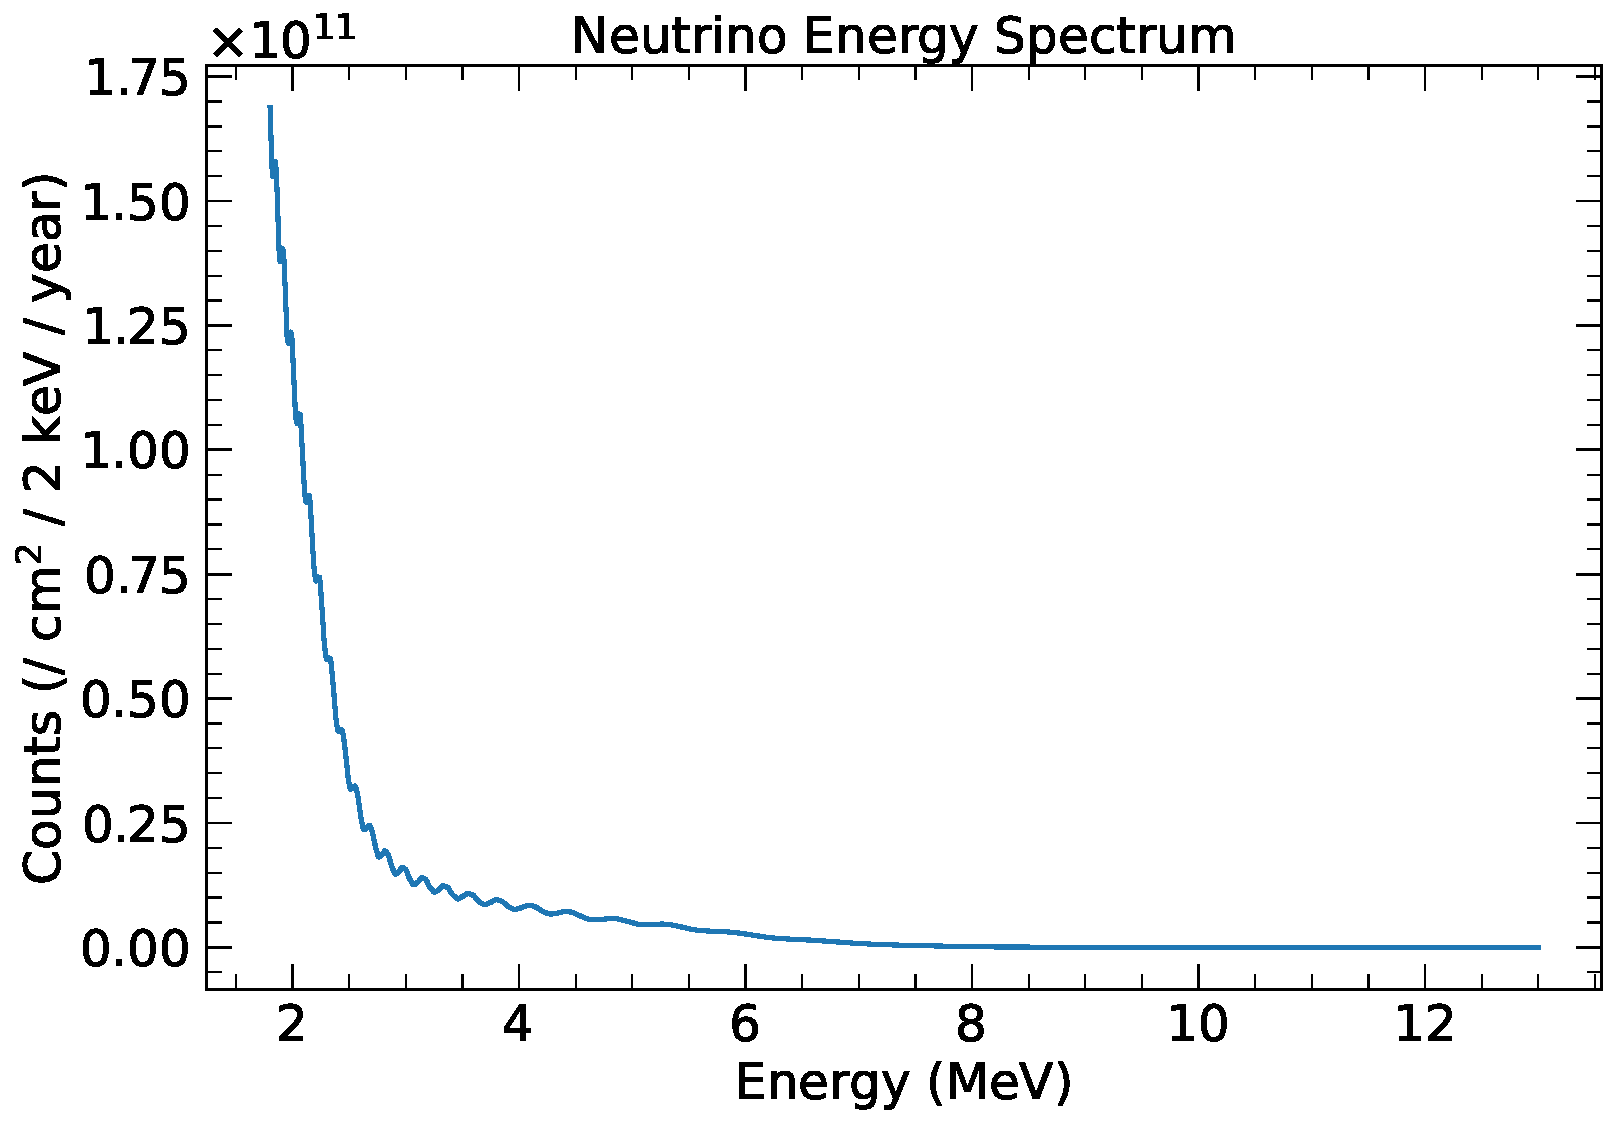
\includegraphics[width=\textwidth]{Img/spectrum_cal/Neutrino_energy_spectrum.pdf}
    \caption{中微子能谱}
    \label{fig:reactor_nu_spectrum}
  \end{subfigure}
  \bicaption{(a) 反应堆发射谱（未加振荡）：按裂变同位素加权并经归一化的电子反中微子能量分布；(b) 加入振荡与几何衰减后的探测器处预期能谱：将发射谱与存活概率以及 $1/4\pi L^2$ 因子相乘并按能量分bin得到的结果（单位为每 cm$^2$ 每年每能量bin计数）。}{(a) Reactor neutrino emission spectrum (no oscillation): the energy-dependent antineutrino yield per fission summed over fissile isotopes and normalized to reactor thermal power. (b) Predicted neutrino spectrum at the detector after oscillation and geometric attenuation: product of the emitted spectrum, oscillation probability and $1/4\pi L^2$ factors, shown here in units of counts per cm$^2$ per year per energy bin.}
\end{figure}



\subsection{沉积能量能谱}  
\label{sec:Deposited energy spectrum}

反应堆释放的反电子中微子能谱 $\phi(E_\nu)$ 通过逆贝塔衰变（IBD）反应与目标质子发生作用，产生正电子并沉积能量。探测到的沉积能量谱 $\phi(E_{\rm dep})$ 可表示为中微子能谱与 IBD 反应截面的卷积：  

\begin{equation}
\label{eq:continuous_rate}
\phi(E_{\rm dep}) \;=\; N_p \,  \int_{1.8}^{13} dE_{\overline{\nu}_e}\; \phi(E_{\overline{\nu}_e}) \; \frac{{\rm d}\sigma}{{\rm d}E_{\rm dep}}(E_{\overline{\nu}_e}, E_{\rm dep})  \; 
\end{equation}

其中 $N_p$ 为探测器中参与反应的自由质子数目，$\phi(E_{\overline{\nu}_e})$ 表示入射反应堆反电子中微子能谱。积分下限 $1.8\,\mathrm{MeV}$ 对应逆贝塔衰变反应的动力学阈值，而上限取 $13\,\mathrm{MeV}$ 以覆盖反应堆反中微子的有效能量范围。  
$\mathrm{d}\sigma/\mathrm{d}E_{\rm dep}(E_{\overline{\nu}_e},E_{\rm dep})$ 为关于沉积能量的 IBD 微分截面，它同时包含了反应截面的能量依赖性以及由散射角和反冲效应引入的动力学映射关系，刻画了给定入射中微子能量 $E_{\overline{\nu}_e}$ 时产生沉积能量 $E_{\rm dep}$ 的微分散射截面。

IBD 反应为 $\bar\nu_e + p \to e^+ + n$，仅当入射反中微子能量超过阈值 $E_{\nu}^{\rm th}\simeq 1.806\ \mathrm{MeV}$ 时才能发生。能量与动量守恒将入射中微子能量 $E_\nu$ 与产生的正电子总能量 $E_{e^+}$ 以及正电子的出射角 $\theta$（定义为中微子方向与正电子方向的夹角）联系起来。在零阶近似下（忽略质子反冲）正电子近似带走 $E_\nu$ 扣除中子–质子质量差 $\Delta=m_n-m_p$ 的能量，湮灭光子与正电子全能共同构成在闪烁体中沉积的能量 $E_{\rm dep}$，因此常用近似 $E_{\rm dep}\simeq E_\nu-0.78\ \mathrm{MeV}$ 作为直观估计。

为了获得更精确的能量映射和角分布权重，本工作采用 Vogel 与 Beacom 给出的 IBD 动力学与微分截面表达式（包括质子反冲等一阶修正及相应的角依赖项）来计算每一对 $(E_\nu,\cos\theta)$ 对应的正电子能量与微分截面 $\mathrm{d}\sigma/\mathrm{d}\cos\theta$（参见文献 \cite{Vogel1999Angular}）。基于该计算，对每个入射能量与发射角的样本点评估其产生的沉积能量并按微分截面加权，从而构造出用于离散化计算的响应矩阵 $M_{ij}$。该矩阵既包含了 IBD 截面的能量依赖性，也反映了由发射角和反冲效应引入的动力学展宽，是将入射中微子谱映射为沉积能量谱的关键数值单元。
\begin{equation}
E_{\rm dep}(E_\nu,\cos\theta)=E_{e^+}(E_\nu,\cos\theta)+m_e
\label{eq:Edep-positron}
\end{equation}
给定 $E_\nu$ 时，不同的 $\cos\theta$ 会产生略有不同的 $E_{\rm dep}$。低能下，IBD 的差分截面可以近似写为 $\frac{d\sigma}{d\cos\theta}\propto 1+v_e\,a(E_\nu)\cos\theta$，其中 $v_e$ 是正电子速率，$a(E_\nu)$ 与 $E_\nu$ 相关~\cite{Vogel1999Angular}。该式意味着在较低能量区，正电子角度分布近似均匀（$d\sigma/d\cos\theta\approx,$常数），只有微弱的方向依赖。基于上述动量学关系，可以将每个入射中微子能量 $E_\nu$ 和对应 $\cos\theta$ 映射到一个 $E_{\rm dep}$ 值，并用于构建响应矩阵。
\begin{equation}
\frac{\mathrm{d}\sigma}{\mathrm{d}E_{\rm dep}}(E_{\bar\nu},E_{\rm dep})
=\int_{-1}^{1}\!\mathrm{d}\cos\theta\;
\frac{\mathrm{d}\sigma}{\mathrm{d}\cos\theta}(E_{\bar\nu},\cos\theta)\;
\delta\!\bigl(E_{\rm dep}-T_e(E_{\bar\nu},\cos\theta)-m_e\bigr)
\label{eq:dsigma-dEdep}
\end{equation}
其中 $E_{\bar\nu}$ 表示入射反电子中微子能量，$T_e$ 为正电子的动力学能（kinetic energy），$m_e$ 为电子静质量。该式将中微子能量与正电子发射角 $\cos\theta$ 映射到可观测的沉积能量 $E_{\rm dep}$：对所有可能的发射角按角分布权重（由微分截面 $\mathrm{d}\sigma/\mathrm{d}\cos\theta$ 给出）进行积分，$\delta$ 函数保证仅在正电子产生的沉积能量恰好等于指定 $E_{\rm dep}$ 时才有贡献。换言之，式中积分把入射能量为 $E_{\bar\nu}$ 的中微子在不同发射角下产生的正电子能量分布累加起来，得到以沉积能量为自变量的微分截面。

物理上，$\mathrm{d}\sigma/\mathrm{d}\cos\theta$ 包含了 IBD 的角分布信息及与能量有关的动力学修正（例如质子反冲、一阶相对论展开项及必要的辐射学修正等；具体公式可参见 VogelBeacom (1999) 等文献）。$\delta$ 函数在理论上给出严格的能量映射，但在数值实现时通常以离散化方式处理：将 $\cos\theta$ 作等距或重要性采样，计算每一采样点对应的 $E_{\rm dep}$，并将该采样点按权重$\mathrm{d}\sigma/\mathrm{d}\cos\theta$ 累加到落入相应沉积能量区间的响应矩阵单元中。若需保留解析上的雅可比因子，可通过对 $\delta\bigl(E_{\rm dep}-T_e(\cos\theta)-m_e\bigr)$ 关于 $\cos\theta$ 的变换引入相应的导数因子；但在常见的蒙特卡洛或格点积分实现中，直接采样并归档权重的方法更加简便且数值稳定。

式中以角分布加权并对 $\cos\theta$ 积分的形式，明确给出了从入射中微子能量到可观测沉积能量的动力学映射关系；在数值实现上，$\delta$ 函数通过对角度采样并按微分截面加权归档到沉积能量区间来近似，从而得到用于后续响应矩阵构造的离散化微分截面。
经离散化后，上述连续映射可写为矩阵形式：
\begin{equation}
S_i \;=\; \sum_j M_{ij}\,\Phi_j,
\label{eq:Si-Mij-Phi}
\end{equation}
其中 $\Phi_j=\Phi(E_{\nu_j})\Delta E_{\nu_j}$ 表示第 $j$ 个中微子能量格点（或能量 bin）上的入射通量积分值，$S_i=S(E_{{\rm dep},i})\Delta E_{{\rm dep},i}$ 表示第 $i$ 个沉积能量格点上的期望事例数。响应矩阵元 $M_{ij}$ 编码了第 $j$ 个中微子能量 bin 的中微子通过 IBD 反应在第 $i$ 个沉积能量 bin 中产生信号的权重（权重包含微分截面、动力学映射與格点宽度等因素）。

在实际构造 $M_{ij}$ 时，常按如下数值流程实现：对每个入射能量格点 $E_{\nu_j}$ 在发射角 $\cos\theta\in[-1,1]$ 上做采样（等距或重要性采样），对每一采样点计算对应的正电子能量并由此得到沉积能量 $E_{\rm dep}=T_e+m_e$。该采样点的贡献按微分截面值 $\mathrm{d}\sigma/\mathrm{d}\cos\theta(E_{\nu_j},\cos\theta_k)$ 加权，并根据 $E_{\rm dep}$ 落入的沉积能量格点 $i$ 将该权重累加到 $M_{ij}$ 上。数值上可表达为求和形式：
\begin{equation}
M_{ij}=\sum_k \frac{\mathrm{d}\sigma(E_{\nu_j},\cos\theta_k)}{\mathrm{d}\cos\theta}\,\Delta\cos\theta\;
\mathbf{1}\bigl(E_{\rm dep}(E_{\nu_j},\cos\theta_k)\in [E_{{\rm dep},i},E_{{\rm dep},i+1})\bigr),
\label{eq:Mij-sum}
\end{equation}
其中 $\Delta\cos\theta$ 是采样步长，$\mathbf{1}(\cdot)$ 为指示函数（若条件成立取 1，否则取 0）。在实现时还常对中微子能量 bin 进行内部细分（sub-sampling）以提高数值精度，且在最终使用前对 $M_{ij}$ 做适当的归一化以符合定义（例如包含 $\Delta E_{\nu}$ 或在乘以 $\Phi_j$ 时一并处理）。

采用上述构造方法得到的响应矩阵自然同时包含了 IBD 微分截面的能量与角度依赖、由发射角和反冲引入的动量学展宽，以及离散化带来的能量混合效应。因此矩阵映射 $S_i=\sum_j M_{ij}\Phi_j$ 在数值上忠实再现了从入射反中微子谱到可观测沉积能量谱的完整物理过程。由基准反应堆通量与构建好的 $M_{ij}$ 得到的典型沉积能量谱示例见图~\ref{fig:depo_e_spec}。

下面给出构建响应矩阵 $M_{ij}$ 的伪代码流程示例（无探测器分辨率等效应），步骤清晰地描述了从中微子能量和角度采样到沉积能量归档的过程：
\begin{algorithm}[htbp]
\caption{生成响应矩阵 $M[i][j]$ 的伪代码}
\begin{algorithmic}[1]
\Require 中微子能量 bins $j$（中心能量 $E_{\nu_j}$），细分 $E_\nu$ 数 $n_{\text{split}}$，余弦角 bin 宽度 $\Delta\cos\theta$
\Ensure 响应矩阵 $M[i][j]$

\ForAll{中微子能量 bin $j$}
  \State $E_{\nu}^{\text{low}} \gets E_{\nu_j}^{\text{left}}$，$E_{\nu}^{\text{up}} \gets E_{\nu_j}^{\text{right}}$，$\Delta E_\nu \gets E_{\nu}^{\text{up}} - E_{\nu}^{\text{low}}$
  \For{$k = 0$ to $n_{\text{split}} - 1$}
    \State $E_{\nu_k} \gets E_{\nu}^{\text{low}} + \left(k + \frac{1}{2}\right) \cdot \frac{\Delta E_\nu}{n_{\text{split}}}$
    \For{$\cos\theta = -1$ to $+1$ step $\Delta\cos\theta$}
      \State 计算正电子动能：$T_1 \gets E_e(E_{\nu_k}, \cos\theta) - m_e$
      \State 计算沉积能量：$E_{\text{dep}} \gets T_1 + 2m_e$，查找 $i$ 使得 $E_{\text{dep}} \in [E_{\text{dep},i}, E_{\text{dep},i+1})$
      \If{找到合法的 $i$}
        \State 计算微分截面：$\frac{d\sigma(E_{\nu_k}, \cos\theta)}{d\cos\theta}$
        \State $\text{weight} \gets \frac{1}{n_{\text{split}}} \cdot \frac{d\sigma}{d\cos\theta} \cdot \Delta\cos\theta$，$M[i][j] \gets M[i][j] + \text{weight}$
      \EndIf
    \EndFor
  \EndFor
\EndFor
\end{algorithmic}
\end{algorithm}




1. 能量分箱：预先定义离散的中微子能量网格和对应的沉积能量网格。
    
2. 角度采样：对每个中微子能量 $E_{\nu_j}$，在 $\cos\theta\in[-1,1]$ 上均匀采样若干点。
    
3. 动量学转换：对每个 $(E_{\nu_j},\cos\theta_k)$，利用 IBD 动量学关系计算正电子全能 $E_{e^+}$，然后得到沉积能量 $E_{\rm dep}=E_{e^+}+m_e$。
    
4. 归档计数：根据 $E_{\rm dep}$ 所在的能量 bin $i$ 将该条事件计入响应矩阵：$M_{ij}+= (d\sigma/d\cos\theta)\Delta\cos\theta$。其中差分截面 $d\sigma/d\cos\theta$ 在每个样本点提供权重，$\Delta\cos\theta$ 是取样间隔。
    
5. 循环累积：对所有中微子能量 bin 和角度样本重复以上过程，最终得到完整的微分散射截面矩阵 $M_{ij}$。
因此微分散射截面矩阵的构建逻辑是先采样中微子能量和出射角度，计算对应的沉积能量，并将相应的微分截面权重累加到正确的能量 bin 中。这样，矩阵 $M_{ij}$ 自动反映了从入射中微子谱到探测沉积谱的完整物理映射关系。
最终，沉积能量能谱可以通过下式得到：
\begin{equation}
\phi_{\rm dep} = \phi_{\nu} \cdot M_{ij}
\label{eq:phi-dep-Mij}
\end{equation}
沉积能量能谱见图~\ref{fig:depo_e_spec}。

\begin{figure}[htbp]
\centering
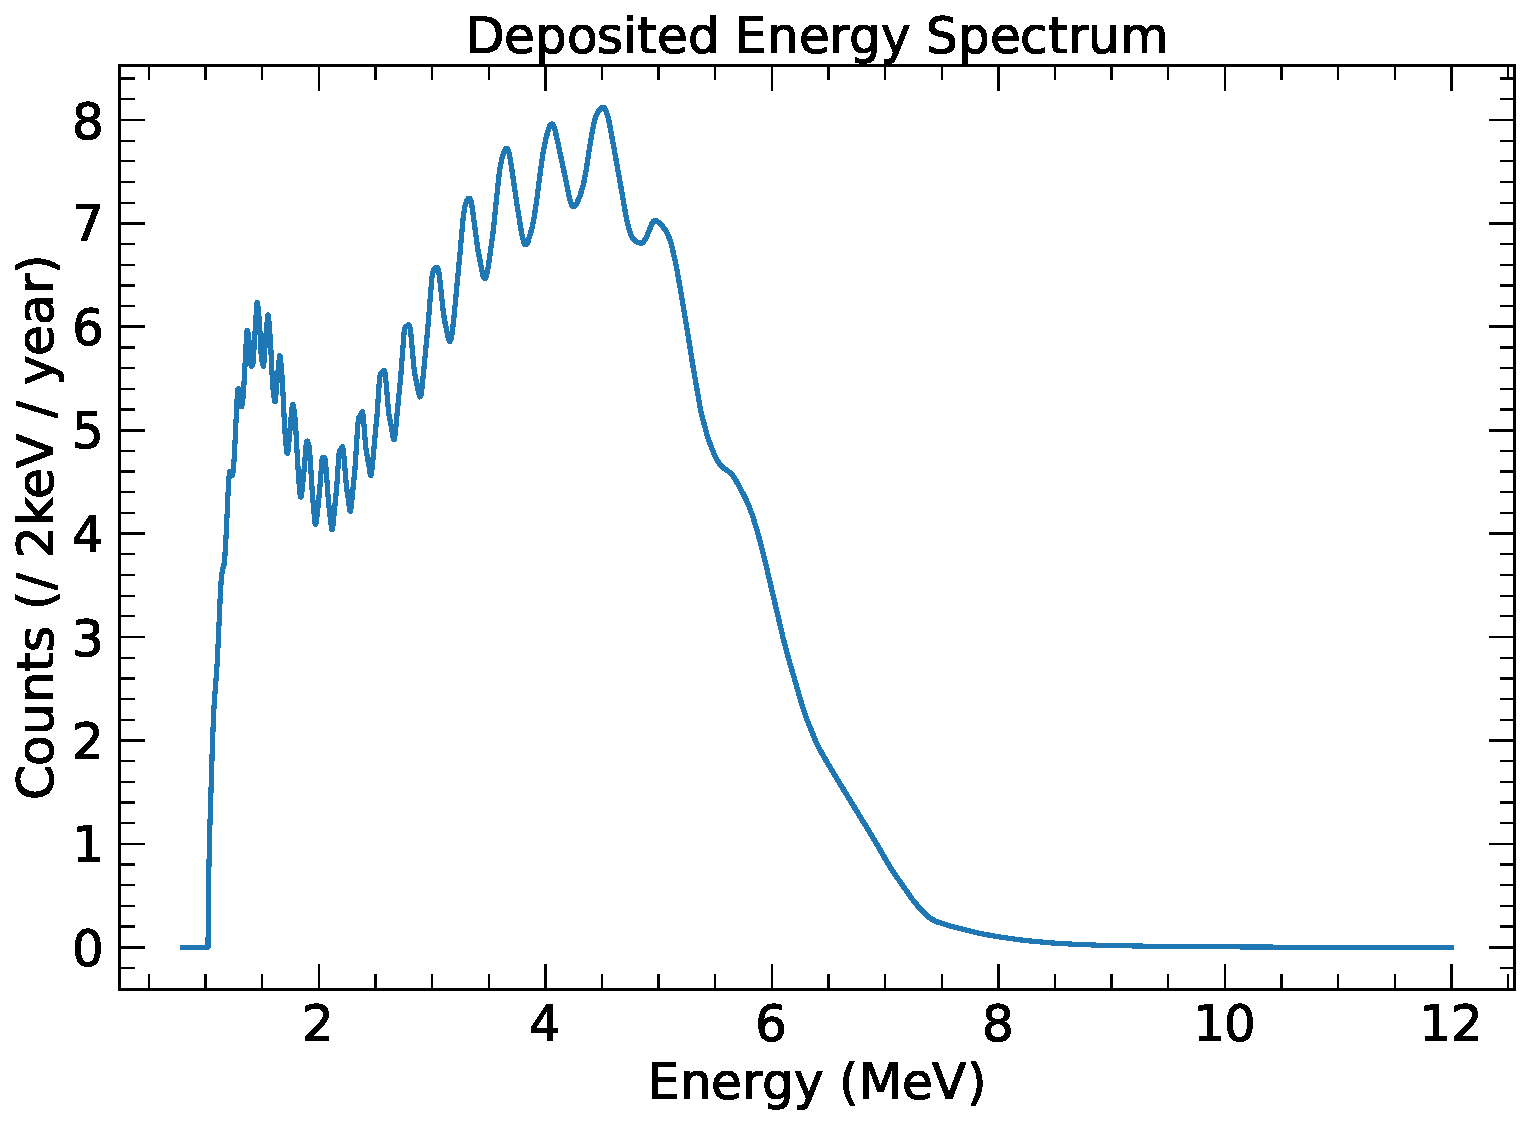
\includegraphics[width=0.6\textwidth]{Img/spectrum_cal/Deposited_energy_spectrum.pdf}
\bicaption{沉积能量能谱}{Deposited energy spectrum}
\label{fig:depo_e_spec}
\end{figure}

\subsection{重建能量能谱}
\label{sec:Reconstructed energy spectrum}
粒子在闪烁体中沉积的能量经过闪烁体本征非线性响应与探测器分辨效应后，最终以重建能量 $E_{\rm rec}$ 的形式被记录下来。重建过程通常分为两步：先将沉积能量映射为可见能量（非线性校正），然后将可见能量以测量误差（能量分辨）随机展宽得到重建能量分布。

首先，闪烁体的非线性响应由经验/校准模型 $f_{\rm LSNL}$ 描述，将沉积能量 $E_{\rm dep}$ 映射为可见能量 $E_{\rm vis}$：  
\begin{equation}  
E_{\rm vis} = E_{\rm dep}f_{\rm LSNL}(E_{\rm dep}) .  
\end{equation}  
函数 $f_{\rm LSNL}(E)$ 随能量变化，涵盖了淬灭（quenching）、Cherenkov 光贡献及其它探测器特异性的非理想效应。通常先通过校准数据确定 $f_{\rm LSNL}$ 的参数与不确定度，得到校正后的期望可见能量记作 $E_{\rm vis}^0$。
可见能量的计算通过下式
\begin{equation}
E_{\rm vis} = E_{\rm dep}\,f_{\rm LSNL}(E_{\rm dep})
\label{eq:Evis-LSNL}
\end{equation}
这里 $f_{\rm LSNL}$ 随沉积能量而变化，将粒子能量损失映射到闪烁光产额。得到 $E_{\rm vis}^0$ 后，还需考虑探测器的能量分辨效应。通常假设分辨函数为高斯型，即重建能量 $E_{\rm rec}$ 服从以均值 $E_{\rm vis}^0$ 为中心的高斯分布，其标准差按经验给出：
\begin{equation}
\sigma_{E_{\rm rec}} = E_{\rm vis} \sqrt{\frac{a^2}{E_{\rm vis}} + b^2 + \frac{c^2}{(E_{\rm vis})^2}}
\label{eq:sigma-Erec}
\end{equation}
其中参数 $a,b,c$ 分别对应光子统计、系统误差和噪声等贡献~\cite{An2021Unfolding}。该形式体现了分辨率随光子计数的泊松涨落、非均匀性和仪器噪声而变化的综合效应。相对分辨率形式~\cite{An2021Unfolding}如下
\begin{equation}
\sigma_{E_{\rm rec}}/E_{\rm vis} = \sqrt{a^2/E_{\rm vis} + b^2 + c^2/E_{\rm vis}^2}
\label{eq:sigma-Erec-rel}
\end{equation}
基于上述处理，可构建探测器响应矩阵 $R_{ij}$，用于将真实的沉积能量谱映射为重建能量谱。具体地，将能量空间离散为一系列能量小区间（bins）。对每个沉积能量小区间 $E_{\rm dep}^{(j)}$，重建能量 $E_{\rm rec}$ 的分布由上述高斯响应给出，因此在第 $i$ 个重构能量区间内出现的概率可由高斯分布的累积分布函数(CDF)计算：
\begin{equation}
\mathrm{CDF}(E_{\rm rec}^{(i)} \mid E_{\rm dep}^{(j)}) = \frac{1}{2}\Bigl[1 + \operatorname{erf}\Bigl(\frac{E_{\rm rec}^{(i)} - E_{\rm vis}}{\sqrt{2}\,\sigma}\Bigr)\Bigr]
\label{eq:CDF-Erec-Edep}
\end{equation}
这里 $\mu=E_{\rm vis}^0$ 为高斯分布均值，$\sigma$ 为上式给出的标准差；$\operatorname{erf}$ 为误差函数，满足 $\frac{1}{2}[1+\operatorname{erf}(x/(\sqrt2))]$ 为标准正态分布的 CDF。由此，第 $j$ 个沉积能量区间映射到第 $i$ 个重建能量区间的概率就是相邻两个阈值之间 CDF 的差值：
\begin{equation}
R_{ij} = \mathrm{CDF}(E_{\rm rec}^{(i+1)} \mid E_{\rm dep}^{(j)}) - \mathrm{CDF}(E_{\rm rec}^{(i)} \mid E_{\rm dep}^{(j)})
\label{eq:Rij-CDF}
\end{equation}
响应矩阵 $R_{ij}$ 既包含由 $f_{\rm LSNL}$ 引起的能量漂移（mean shift），也包含由能量分辨引起的展宽（smearing），能够准确描述沉积能量向重建能量的转换概率分布。
最终，任意给定的沉积能量谱 $\Phi_{\rm dep}(E_{\rm dep,j})$ 与响应矩阵相乘即可得到对应的重建能量能谱 $\Phi_{\rm rec}(E_{\rm rec,i})$：
\begin{equation}
\phi_{\rm rec}(E_{\rm rec,i}) = \sum_j R_{ij}\,\phi_{\rm dep}(E_{\rm dep,j})
\label{eq:phi-rec-Rij}
\end{equation}
通过将沉积能量谱与高斯响应函数卷积得到重建能量谱,见图~\ref{fig:recons_e_spec}：体现了探测器对原始中微子能谱的响应，即通过能量非线性校正和分辨率展宽对真实能量谱进行smearing”，从而得到可与实验数据直接比较的重建能谱。
通过将闪烁体中的能量淬火和光统计涨落等效应分离开来，先通过非线性修正得到理想可见能量，再通过高斯分布描述测量误差，最终通过响应矩阵系统地将理论沉积谱映射到实验观测谱，对中微子能谱的精确重建至关重要。
\begin{figure}[htbp]
\centering
\includegraphics[width=0.6\textwidth]{Img/spectrum_cal/Reconstructed_energy_spectrum.pdf}
\bicaption{重建能量能谱}{Reconstructed energy spectrum}
\label{fig:recons_e_spec}
\end{figure}
反应堆中微子能谱与重建能谱关系可写为：flux $\to$ cross-section $\to$ detector response $\to$ reconstruction。
\begin{equation}
N_{\text{reco}}(E_{\text{reco}})=
\int R(E_{\text{reco}},E_{\text{true}})\,
N_{\text{true}}(E_{\text{true}})\,\mathrm{d}E_{\text{true}}.
\label{eq:Nreco-response}
\end{equation}

\section{统计拟合方法}

我们基于分箱的重构能谱来进行振荡参数估计。设由振荡参数 $\theta$ 与一组系统不确定性（赘余）参数 $\alpha$ 所决定的理论预测分箱重建能谱谱为$\boldsymbol{T}(\theta,\alpha)$。其中 $\theta=(\sin^2\theta_{12},\Delta m^2_{21},\Delta m^2_{31},\sin^2\theta_{13})$。观测数据记为向量 $\boldsymbol{M}$（JUNO 的分箱观测能谱）。为同时考虑统计不确定性与多种系统误差，我们采用含拉项（pull terms）的最小二乘（$\chi^2$）方法构造目标函数并进行拟合，其一般化的表达式如式~\ref{chisq}所示。

\begin{equation}
  \chi^2 \equiv(\boldsymbol{M}-\boldsymbol{T}(\boldsymbol{\theta}, \boldsymbol{\alpha}))^T \cdot \boldsymbol{V}^{-1} \cdot(\boldsymbol{M}-\boldsymbol{T}(\boldsymbol{\theta}, \boldsymbol{\alpha}))+\sum_k\left(\frac{\alpha_k}{\sigma_k}\right)^2,
  \label{chisq}
  \end{equation}
将式~\ref{chisq}展开可得到完整形式~\ref{chisq_complete}，
JUNO 的 χ² 由数据项（残差平方和）与一系列表示系统不确定性的惩罚项（Gaussian pull）组成，形式为  
\begin{equation}
\begin{aligned}
\chi^2 \equiv\; & \sum_i^{N_{\rm bins}}\left(\frac{\left(M_i-T_i^{\mathrm{IBD}}(\boldsymbol{\alpha})-\sum_B^{\mathrm{Bkg}}\left[T_i^B \left(1+\alpha_B\right)\right]\right)^2}{\left(T_i^{\mathrm{IBD}}(\boldsymbol{\alpha})+\sum_B^{\mathrm{Bkg}} T_i^B\right)+\left(T_i^{\mathrm{IBD}}(\boldsymbol{\alpha}) \, \sigma_{\mathrm{shp}}^i\right)^2+\sum_B^{\mathrm{Bkg}}\left(T_i^B \, \sigma_{\mathrm{shp}}^B\right)^2}\right) \\
& + \left(\frac{\alpha_C}{\sigma_C}\right)^2
  + \sum_{r}^{\mathrm{Cores}}\left(\frac{\alpha_r}{\sigma_r}\right)^2
  + \left(\frac{\alpha_D}{\sigma_D}\right)^2
  + \sum_B^{\mathrm{Bkg}}\left(\frac{\alpha_B}{\sigma_B}\right)^2
  + \sum_{l=1}^4\left(\frac{\alpha_l}{\sigma_l}\right)^2 \\
& + \left(\frac{\alpha_{\mathrm{EScale}}}{\sigma_{\mathrm{EScale}}}\right)^2
  + \sum_{p}^{\mathrm{NPP}}\left(\frac{\alpha_{{\mathrm{Pow}},p}}{\sigma_{{\mathrm{Pow}},p}}\right)^2
  + \sum_{\eta=a, b, c}\left(\frac{\alpha_\eta}{\sigma_\eta}\right)^2
  + \left(\frac{\alpha_{\rho \mathrm{ME}}}{\sigma_{\rho \mathrm{ME}}}\right)^2 \\
& + \sum_{p}^{\mathrm{NPP}}\left(\frac{\alpha_{\mathrm{SNF},p}}{\sigma_{\mathrm{SNF},p}}\right)^2
  + \sum_{p}^{\mathrm{NPP}}\left(\frac{\alpha_{\mathrm{Non\mbox{-}Eq},p}}{\sigma_{\mathrm{Non\mbox{-}Eq},p}}\right)^2
  + \left(\frac{\alpha_{\mathrm{Th/U}}}{\sigma_{\mathrm{Th/U}}}\right)^2
  + \sum_{f}^{\mathrm{FF}}\left(\frac{\alpha_{{\mathrm{FF}},f}}{\sigma_{{\mathrm{FF}},f}}\right)^2
  + \sum_{f}^{\mathrm{FE}}\left(\frac{\alpha_{{\mathrm{FE}},f}}{\sigma_{{\mathrm{FE}},f}}\right)^2 \, ,
\end{aligned}
\label{chisq_complete}
\end{equation}
其中第一行为分箱数据项，分母包含统计方差与若干背景谱形不确定度项；第二行及后续项为对各类系统不确定性的 Gaussian 约束（拉项）。相关符号及赘余参数（pull parameters）的含义在下文“数据项符号说明”和“系统不确定性 pull term”两小节中统一列出。
\subsubsection*{数据项符号说明}

\begin{itemize}
  \item $i$：重建能量谱中的第 $i$ 个能量 bin。
  \item $M_i$：第 $i$ 个重构能量 bin 中的观测事件数（信号+背景）。
  \item $T_i^{\mathrm{IBD}}(\theta,\alpha)$：预测的 IBD 信号事件数，依赖振荡参数与各类系统参数。
  \item $T_i^{B}(\alpha_B)$：第 $B$ 类背景在第 $i$ 个 bin 中的预测值。
  \item $V_{ii}^{\mathrm{stat}}$：统计方差估计（见式~\eqref{eq:Chisq:CNP}）。
  \item $\sigma_{\mathrm{shp}}^B$：第 $B$ 类背景的谱形不确定度。
  \item $f$：裂变同位素索引，分别对应 $^{235}$U、$^{238}$U、$^{239}$Pu、$^{241}$Pu。
\end{itemize}

\subsubsection*{系统不确定性pull term}

各赘余参数（pull term）及其物理含义如下：

\begin{itemize}
  \item \textbf{反应堆与探测器整体归一化}
    \begin{itemize}
      \item $C$：反应堆相关的整体相关不确定性，用于描述所有反应堆共同的通量归一化偏差（如反应堆反中微子通量模型的不确定性）。
      \item $D$：探测效率不确定性，对应 IBD 事件整体探测效率（包括触发、选择效率等）的归一化误差。
      \item P：反应堆热功率不确定性，直接影响反中微子产生率的整体归一化。
      \item FE：裂变能量（fission energy）不确定性，影响由热功率换算得到的反中微子通量归一化。
      \item FF：四种裂变同位素的裂变份额（fission fractions）不确定性，采用协方差矩阵 $\rho_{\mathrm{FF}}$ 刻画其相关性。
    \end{itemize}
  \item \textbf{能量响应相关}
    \begin{itemize}
      \item EScale：绝对能量刻度不确定性，描述探测器能量标定整体偏移对重建能谱的影响。
      \item $l$：第 $l$ 条液体闪烁体非线性（LSNL）拉曲线参数，用于刻画能量非线性模型的不确定性对谱形的影响。
      \item $\eta=(a,b,c)$：能量分辨率参数，对应能量分辨率经验公式中光子统计项、非均匀性项和电子噪声项的不确定性。
      \item shp：能谱形状不确定性，用于描述反应堆反中微子谱或背景谱的 bin-to-bin 形变。
    \end{itemize}
  \item \textbf{本底相关}
    \begin{itemize}
      \item $B$：第 $B$ 类本底过程（如偶然符合本底、Bi-Po214，宇宙线次级粒子、大气中微子等），用于描述不同本底rate不确定度。
      \item Th/U：地球反中微子中 Th 与 U 同位素贡献比例的不确定性。
    \end{itemize}
  \item \textbf{反应堆运行相关}
    \begin{itemize}
      \item $p$：第 $p$ 座核电站，用于区分来自不同核电站的功率、乏燃料等不确定性。
      \item NonEq：非平衡修正项不确定性，反映短寿命裂变产物未达到平衡状态对反应堆反中微子谱的影响。
      \item SNF：乏核燃料（Spent Nuclear Fuel）不确定性，用于描述反应堆停堆后燃料产生的额外反中微子通量。
    \end{itemize}
  \item \textbf{物质效应}
    \begin{itemize}
      \item $\rho_{\mathrm{ME}}$：地球物质密度不确定性，用于刻画物质效应（matter effect）对振荡概率的修正。
    \end{itemize}
\end{itemize}
为兼顾 Neyman（$\sigma^2\approx M$）与 Pearson（$\sigma^2\approx T$）估计在低计数箱中的偏差问题，我们采用加权组合的统计方差（CNP 组合）：  
\begin{equation}  
V_{ii}^{\rm stat} \equiv 3\left(\frac{1}{M_i}+\frac{2}{T_i^{\rm IBD}+\sum_B T_i^{B}}\right)^{-1}.  
\label{eq:Chisq:CNP}  
\end{equation}  
该组合在数值上消除了 Neyman 与 Pearson 各自的第一阶偏倚，并能避免零计数箱导致的分母为零的问题，从而在近似泊松极限下改善参数估计的稳健性。
$\chi^2$的最小化采用 \texttt{iminuit} 软件包中的 MIGRAD 算法完成，该算法基于拟牛顿法和梯度信息，具有良好的收敛速度与数值稳定性。当期望最小化距离（EDM）低于设定阈值后，迭代终止并认为拟合收敛。通过对冗余参数进行剖面化（profiling），得到物理参数的最优估计及其不确定度。

\subsection{Wilks 定理与 Feldman–Cousins 方法}  
\label{sec:statistical method}

在高能物理与中微子数据分析中，参数置信区间的估计通常基于检验统计量 $\Delta\chi^2$ 的统计行为。Wilks 定理~\cite{Wilks:1938dza}在大样本极限下为构造置信区间提供了方便的近似：在满足一定正则条件的情形下（例如假设为嵌套、参数为内点且样本量充分大），一维情形下的检验统计量
\begin{equation}
\Delta\chi^2(\delta)=\chi^2(\delta)-\chi^2_{\min}
\label{eq:Delta-chi2}
\end{equation}
近似服从自由度为 1 的 $\chi^2$ 分布。因此，可以使用固定阈值来构造置信区间，例如 $\Delta\chi^2=1$ 对应约 68.27\% 的置信水平，从而实现高效的区间估计。

但是，Wilks 定理的适用依赖于若干正则条件，这些条件在反应堆与加速器中微子实验中并不总是成立。常见会破坏 Wilks 定理近似的情形包括：参数有边界（bounded parameters）、参数空间的非光滑或非正则性、似然面存在多重或不相连的极小值（由参数简并或谱形-振荡耦合引起）、以及样本量不足使渐近性质失效~\cite{Acero2022ProfiledFC,Ogawa1964}等。在这些非正则条件下，$\Delta\chi^2$ 的经验分布会偏离理想的 $\chi^2$ 分布，导致用固定 $\Delta\chi^2$ 阈值构造的置信区间不再具有名义上的覆盖率（coverage）保证。需要指出的是，低统计并非 Wilks 失效的唯一原因，但会放大非正则效应并使偏差更加显著~\cite{Cordeiro1995}。

为了解决上述问题并保证频率学意义上的正确覆盖率，可采用 Feldman–Cousins（FC）方法~\cite{Feldman_1998}。FC 方法的核心思想是通过大量伪实验（toy Monte Carlo）直接构造检验统计量在假设参数值下的经验分布，从而得到参数依赖的临界值 $\Delta\chi^2_{\rm crit}(\delta)$。具体地，对于每个假定参数点 $\delta_i$，生成大量基于该 $\delta_i$ 的伪数据样本并计算相应的检验统计量分布，然后在所需置信水平下取出临界值。实际数据在该点的 $\Delta\chi^2(\delta_i)$ 若不超过 $\Delta\chi^2_{\rm crit}(\delta_i)$，则该参数点被包含于构造的置信区间内。由于临界值是通过模拟获得的，FC 构造在参数受界、非正则或多峰情形下仍能保证所设置信度的频率学覆盖性。

然而，FC 方法的代价是显而易见的：要构建完整的一维（或更高维）参数相关的置信带，必须在多个参数点 $\{\delta_i\}$ 上分别生成大量伪实验并计算临界值；当问题包含大量赘余参数（nuisance parameters）或考察高维参数空间时，所需的计算量会呈指数级增长。对于需要在不同谱形假设、不同能谱分 bin、不同系统扰动下重复评估的反应堆拟合任务而言，这种计算负担尤其沉重，常常成为高精度统计推断中的主要瓶颈。

基于上述考量，反应堆中微子实验的数据分析不仅需要严谨的统计方法论（如在必要时使用 FC 以保证覆盖），还迫切要求构建高效、可扩展的谱拟合与伪实验生成框架。常见的加速手段包括但不限于：将谱预测與似然评估张量化以减少解释性语言的循环开销、对响应矩阵与中间结果进行缓存与稀疏化存储、对伪实验并行化调度（多核/集群/GPU）、采用重要性抽样或代理模型（surrogate model）在参数空间中近似临界值曲线、以及对冗余参数实施剖面化插值（profiling interpolation）以减少重复拟合次数。后续章节将详细介绍本工作中所实现的若干加速策略以及其在大规模 FC 构造与 toy-MC 研究中的性能表现。

\section{本章总结}
本章系统介绍了反应堆中微子振荡分析的理论与数值框架，为后续灵敏度研究与覆盖率检验奠定了基础。围绕“从反应堆到重建谱”的分析主线，本章在物理建模、数值实现与统计推断三个层面取得了以下结果。

在物理层面，本章介绍了从反应堆反中微子的产生、传播与 IBD反应，最后到探测器探测到的重建能量能谱，明确给出了从入射中微子能谱到重建能量能谱的映射关系，并系统刻画了微分截面、能量转换关系以及探测器非线性与能量分辨模型对谱形的影响。

在数值实现层面，本章的构建了张量化的谱生成框架。通过将反应堆能谱、IBD 微分截面矩阵、沉积能量转换以及探测器响应矩阵统一表示为高维张量运算，实现了谱生成流程的模块化与矩阵化表达。该实现方式在保持物理透明性的同时显著提升了计算效率与可扩展性，使多参数扫描、批量 toy-MC 生成以及协方差传播能够在统一框架下完成。

在统计推断层面，本章介绍了含pull term的 $\chi^2$ 构造形式，系统纳入反应堆、探测器与本底相关的不确定性来源，并采用 CNP 统计方差组合以降低低计数区间的偏倚问题。同时讨论了 Wilks 定理的适用条件与局限性，指出在非正则情形下需要借助 Feldman–Cousins 方法进行严格覆盖率评估，从而明确了后续加速拟合算法研究的必要性。

总体而言，本章完成了反应堆中微子振荡分析链条的形式化与数值化构建，实现了一个可计算、可扩展且物理自洽的拟合框架。这一框架不仅支持振荡参数的精确提取，也为后续章节中对计算效率优化与统计覆盖率检验的深入研究提供了坚实基础。
